\documentclass[slidestop,compress,mathserif, aspectratio = 169]{beamer}
\usetheme[block = fill, numbering = none]{metropolis}
\usepackage{etex}
\useinnertheme{rectangles}
\usepackage{graphicx}
\usepackage{subfig}
\usepackage{epigraph}
\usepackage{makeidx}
\usepackage[]{amsmath}
\usepackage[]{amssymb}
\usepackage{color}
\usepackage{pict2e}
\usepackage{algorithm2e}
\usepackage[ngerman]{babel}
\usepackage{tikz}
\usetikzlibrary{mindmap}
\usepackage{multirow}
\usepackage{ulem}
\usepackage[utf8]{inputenc}
\usepackage{multimedia}
\usepackage{xcolor}
\usepackage{keyval}
\usepgfmodule{shapes}
\usepackage{pgfplots}
\usepackage{sansmath}
\usepackage{pgfgantt}
\usetikzlibrary{arrows}
\usetikzlibrary{graphs, automata, spy, positioning}
\usetikzlibrary{shapes.gates.logic.US,trees}
\usepackage{colortbl}
\usepackage{array}
\usepackage{listings}
\usepackage{pdfpages}
\usepackage{textcomp}
\pgfplotsset{width=6cm}


%\definecolor{RYB1}{RGB}{240,249,232}
%\definecolor{RYB2}{RGB}{186,228,188}
%\definecolor{RYB3}{RGB}{123,204,196}
%\definecolor{RYB4}{RGB}{67,162,202}
%\definecolor{RYB5}{RGB}{18,104,172}
%
%\definecolor{blue}{rgb}{0,0,1}
%\definecolor{mint}{cmyk}{75,0,40,0}
%\definecolor{mint}{rgb}{32,178,170}
\graphicspath{{./WebApp/figures/}}

\mode<handout>{
\usepackage{pgfpages}
\pgfpagesuselayout{2 on 1}[a4paper,border shrink=5mm]
}

\AtBeginSection{\frame{\sectionpage}}
\AtBeginSubsection{\frame{\subsectionpage}}
\newtranslation[to=ngerman]{Section}{Teil}
\newtranslation[to=ngerman]{Subsection}{Abschnitt}

\setbeamersize{text margin left=.8cm, text margin right=.8cm}

%\setbeamertemplate{frametitle}{%
%    \nointerlineskip%
%    \begin{beamercolorbox}[wd=\paperwidth,ht=2.0ex,dp=0.6ex]{frametitle}
%        \hspace*{1ex}\insertframetitle%
%    \end{beamercolorbox}%
%}

\newcommand\MyBox[2]{
  \fbox{\lower0.75cm
    \vbox to 1.7cm{\vfil
      \hbox to 1.7cm{\hfil\parbox{1.4cm}{#1\\#2}\hfil}
      \vfil}%
  }%
}

\pgfmathdeclarefunction{norm}{3}{%
                      \pgfmathparse{sqrt(0.5*#3/pi)*exp(-0.5*#3*(#1-#2)^2)}%
                    }
\begin{document}

\setbeamertemplate{bibliography item}{\insertbiblabel}
\tikzstyle{element} = [draw,rectangle, align = center, text width = 2.5 cm, node distance = 1.25 cm]

% Formalia
\newcommand{\Var}{\operatorname{Var}}
\newcommand{\mum}{\operatorname{\mu m}}
\newcommand{\E}{\operatorname{E}}
\newcommand{
\offslide}[2]{
\begin{frame}
\frametitle{\includegraphics[scale=0.05] {Offwhite} \hspace{.5mm} #1}
%\framesubtitle{#2}
\begin{tikzpicture}[x=1cm, y=1cm, semitransparent]
\draw[step=5mm, line width=0.2mm, black!40!white] (0,0) grid (\textwidth,\textheight-1cm);
\node[anchor = south east] at (\textwidth,0) {#2};

\end{tikzpicture}
\end{frame}
}
\newcommand{\source}[1]{\rotatebox{90}{\tiny \color{gray} #1}}

\newcommand{\lehrtext}[1]{
\only<article>{
\vspace{0.3cm}
\leavevmode%
  \tabto*{-1.8cm}% LEFT MARGIN
  %\tabto*{\dimexpr\linewidth+40pt\relax}% RIGHT MARGIN
  \smash{\belowbaseline[-\ht\strutbox]{\makebox[0pt]%
%    [r]% LEFT MARGIN
    [l]% RIGHT MARGIN
  {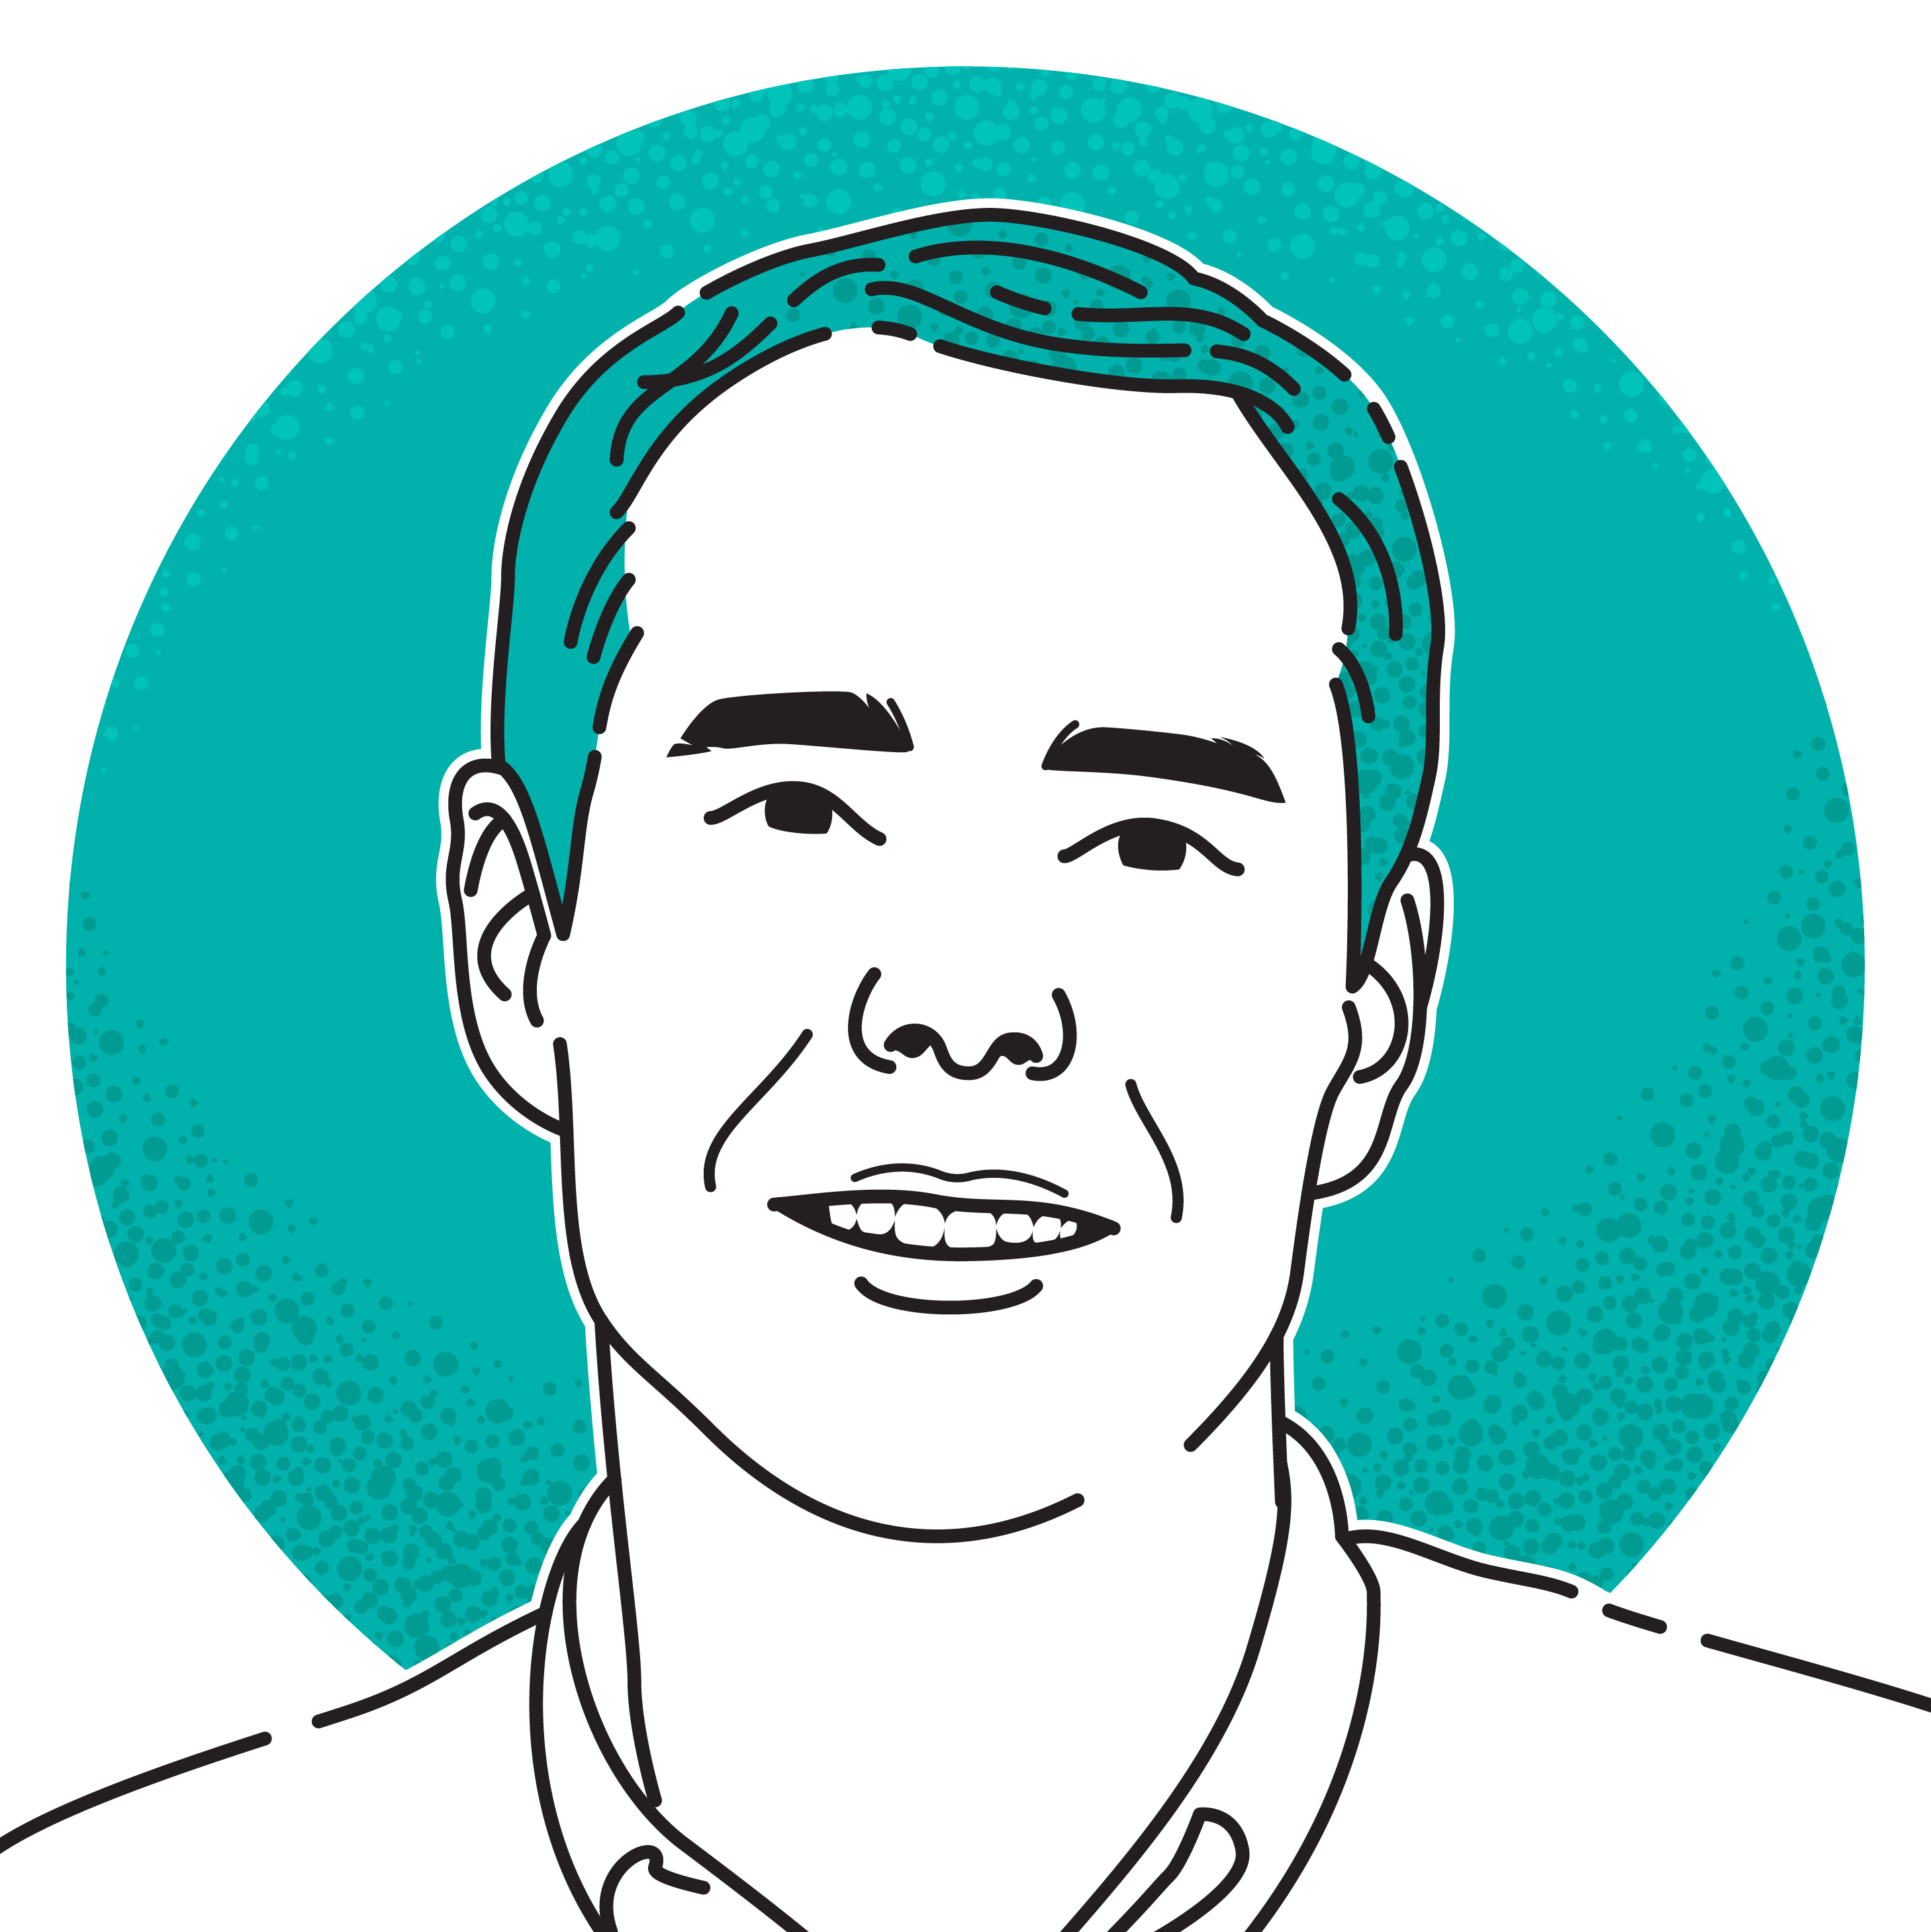
\includegraphics[width = 1.5cm]{teacher}}}}%
  \tabto*{\TabPrevPos}%
#1
}
}

\title{Rail Data Science}
\subtitle{Deployment to a WebApp}
\author{Prof. Dr. Raphael Pfaff}
\institute[FH Aachen]{Fachhochschule Aachen}
\logo{\put(-18, 120){
\includegraphics[width=1.4cm]{logoR}}}

\begin{frame} % Cover slide
\titlepage
\end{frame}
\frame{\frametitle{Framework: Flask}
     	\begin{itemize}
		\item Microframework: 
		\begin{itemize}
			\item No tools or libraries required
			\item Easy to use for non-critical applications
		\end{itemize}
		\item Concepts:
		\begin{itemize}
			\item Instantiate Flask
			\item App routing to different endpoints
		\end{itemize}
		\item Can be used together with Plotly for interactive plot delivery
     	\end{itemize}
   }

\lstdefinestyle{mystyle}{
%    backgroundcolor=\color{backcolour},   
    commentstyle=\color{mLightGreen},
 %   keywordstyle=\textbf\color{mDarkTeal},
    %numberstyle=\tiny\color{codegray},
    stringstyle=\color{mLightBrown},
%    basicstyle=\ttfamily\footnotesize,
%    breakatwhitespace=false,         
%    breaklines=true,                 
%    captionpos=b,                    
%    keepspaces=true,                 
%    numbers=left,                    
%    numbersep=5pt,                  
%    showspaces=false,                
%    showstringspaces=false,
%    showtabs=false,                  
%    tabsize=2
}

\lstset{style=mystyle}

\frame{\frametitle{Import in WebApp (app.py)}
     	\lstinputlisting[language=Python, firstline = 1, lastline = 13]{WebApp/App/app.py}
   }
   
 \frame{\frametitle{Create app}
     	\lstinputlisting[language=Python, firstline = 15, lastline = 16]{WebApp/App/app.py}
   }

\begin{frame}[allowframebreaks]\frametitle{Preload data}
	Preloading of data at startup of the app speeds up the app significantly. For this we use the app route @app.before\_first\_request:
     	\lstinputlisting[language=Python, firstline = 18, lastline = 32]{WebApp/App/app.py}
   \end{frame}
   
   \begin{frame}[allowframebreaks]\frametitle{Plot time series data}
   \begin{enumerate}
	\item  Define app route and and function:
     	\lstinputlisting[language=Python, firstline = 34, lastline = 35]{WebApp/App/app.py}
	\item Open an error catching environment:
	\lstinputlisting[language=Python, firstline = 36, lastline = 36]{WebApp/App/app.py}
	\item Declare the dataframe as global:
	\lstinputlisting[language=Python, firstline = 37, lastline = 37]{WebApp/App/app.py}
	\item Generate the plot:
	\lstinputlisting[language=Python, firstline = 38, lastline = 47]{WebApp/App/app.py}
	\item Transform the plot into a HTML div:
	\lstinputlisting[language=Python, firstline = 48, lastline = 51]{WebApp/App/app.py}
	\item Render as HTML page, transferring the plotcode:
	\lstinputlisting[language=Python, firstline = 52, lastline = 52]{WebApp/App/app.py}
	\newpage
	\item Catch the exception:
	\lstinputlisting[language=Python, firstline = 53, lastline = 55]{WebApp/App/app.py}
	\end{enumerate}
	
   \end{frame}
   
   \frame{\frametitle{Start the app}
     	\lstinputlisting[language=Python, firstline = 106, lastline = 104]{WebApp/App/app.py}
   }
   
    \begin{frame}[allowframebreaks]\frametitle{A geospatial plot on a different app route and in a different function}
     	\lstinputlisting[language=Python, firstline = 58, lastline = 104]{WebApp/App/app.py}
   \end{frame}

\frame{\frametitle{Start the app}
\begin{columns}[t] 
     \begin{column}[T]{7cm} 
     	\begin{itemize}
		\item \texttt{cd} to App directory
		\item \texttt{python app.py}
		\item Apps works on localhost
     	\end{itemize}
     \end{column}
     	\begin{column}[T]{7cm} 
         	\begin{center}
            		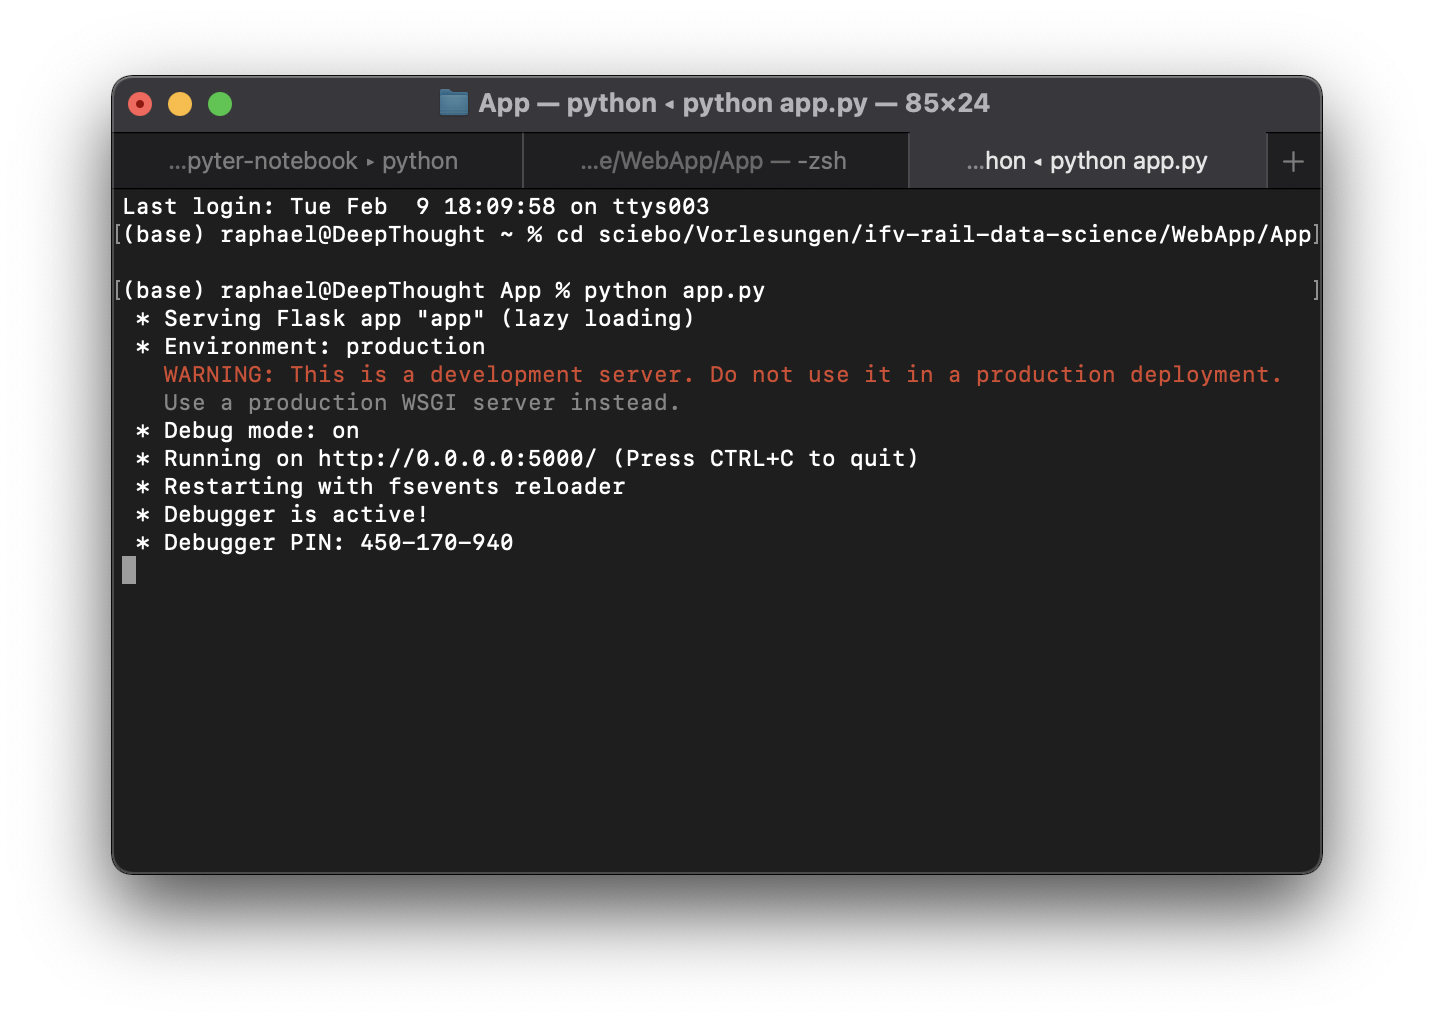
\includegraphics[width=0.95\textwidth]{startApp}\source{}
        		\end{center}
     \end{column}
 \end{columns}
}

\frame{\frametitle{Run the app}
\begin{columns}[t] 
     \begin{column}[T]{7cm} 
     	\begin{itemize}
		\item In a browser, visit \\
		\texttt{localhost:5000} \\
		and
		\item \texttt{localhost:5000/geo}
     	\end{itemize}
     \end{column}
     	\begin{column}[T]{7cm} 
         	\begin{center}
            		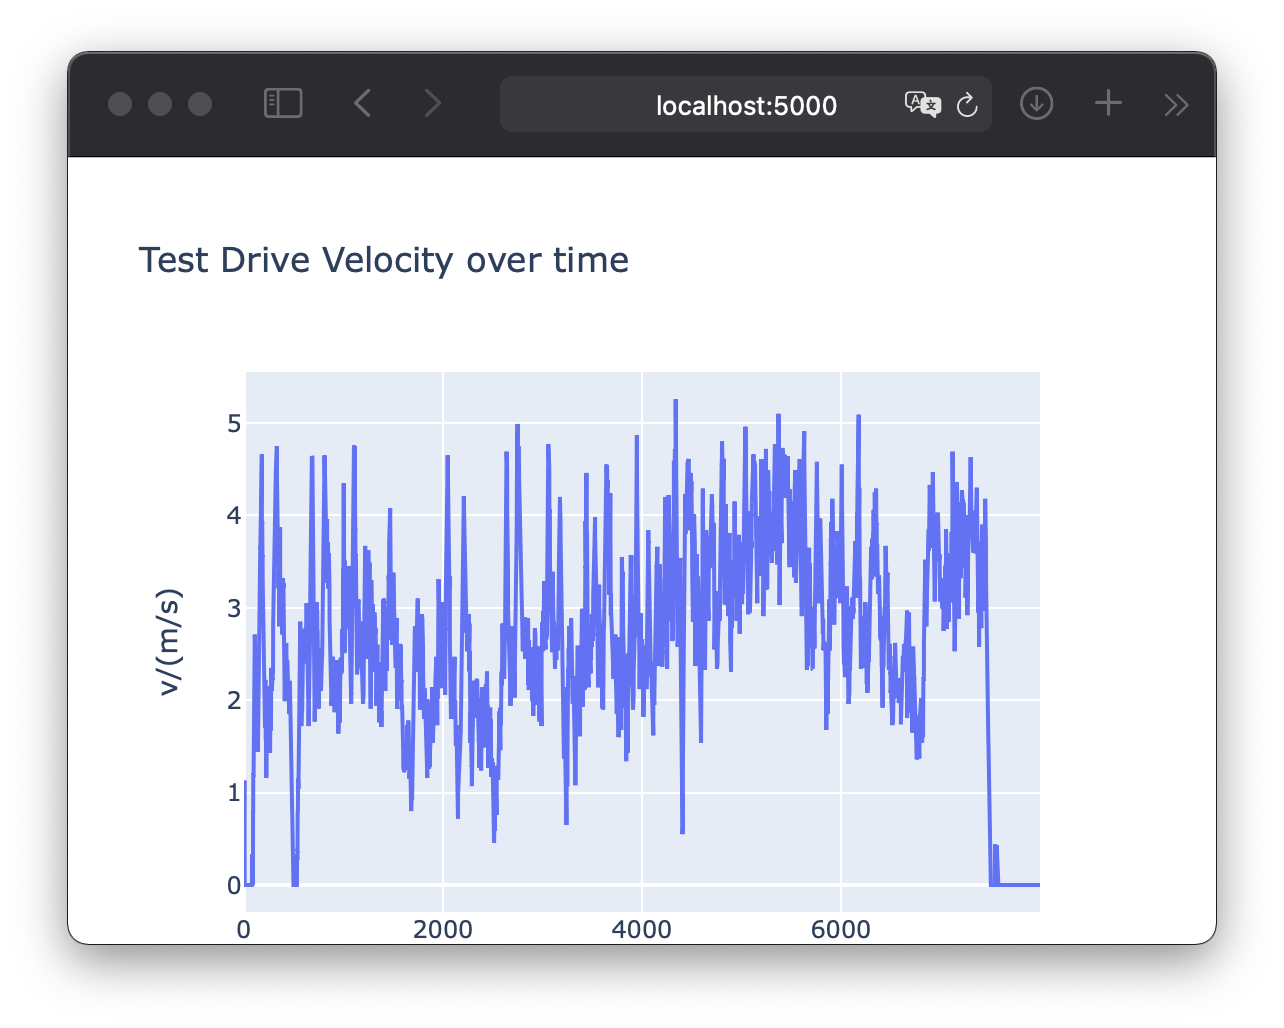
\includegraphics[width=0.55\textwidth]{App}\source{}
		\begin{flushright}
		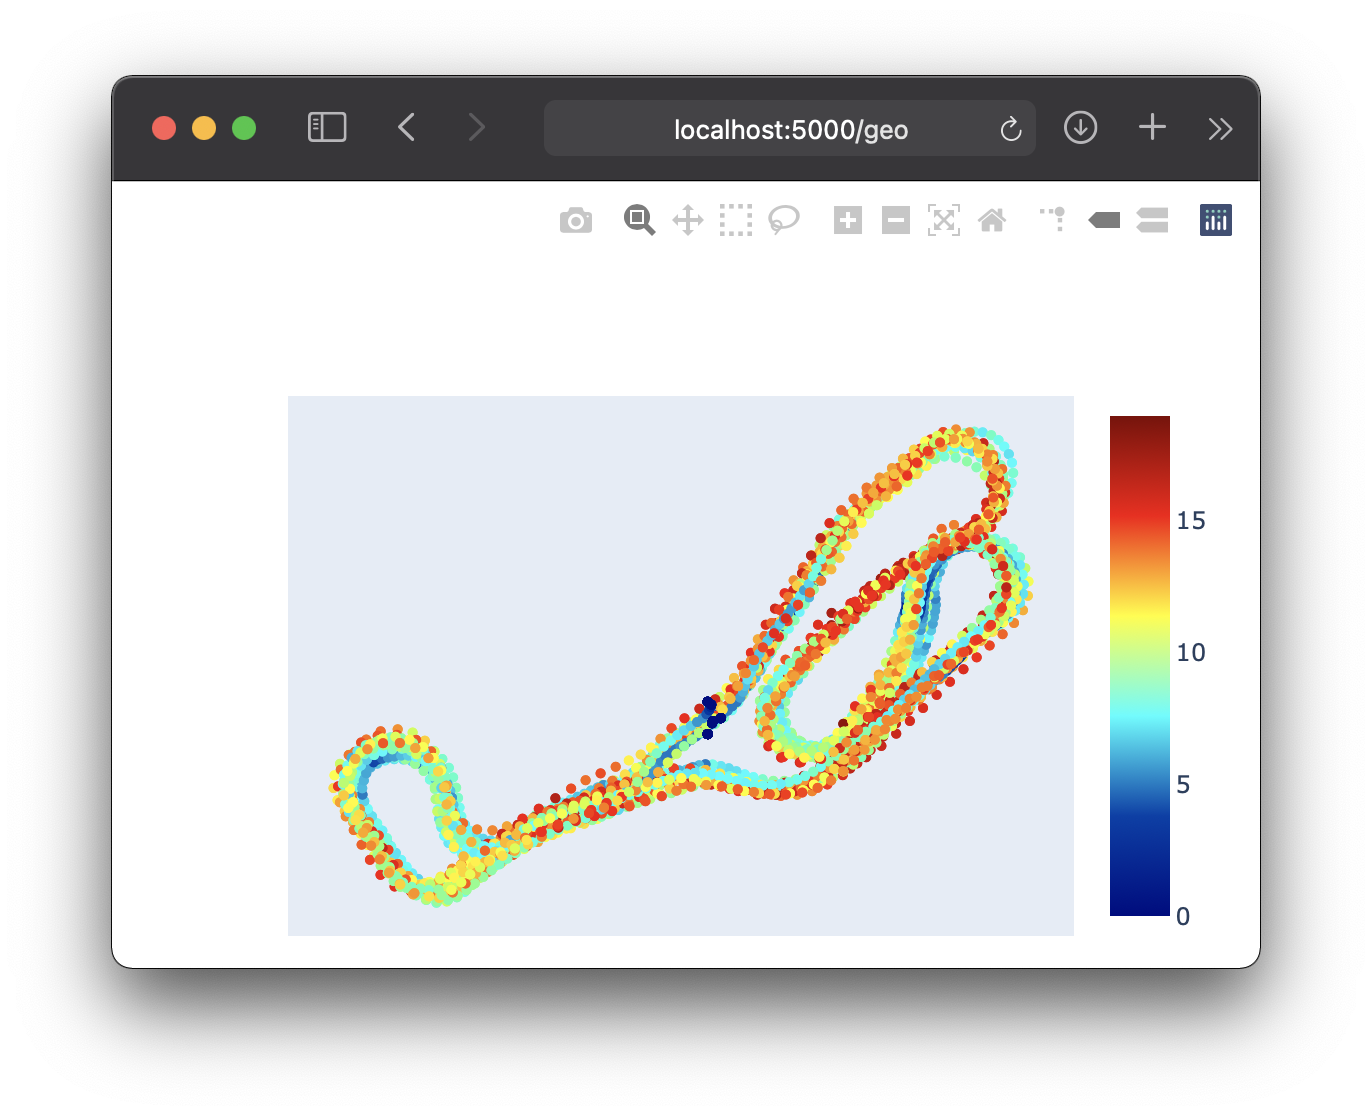
\includegraphics[width=0.55\textwidth]{Appgeo}\source{}
		\end{flushright}
        		\end{center}
     \end{column}
 \end{columns}
}

\frame{\frametitle{Exercise}
     	\begin{itemize}
		\item Extend the web app by adding another route \texttt{/hist} that delivers a plotly histogram
		\begin{itemize}
			\item To generate a histogram, use \texttt{data = go.histogram(x = df['v'])}
			\item The remainder of the plot code can stay mostly the same
		\end{itemize}
     	\end{itemize}
   }


\end{document}
